% =============================================================================
% Episode 023: Visual Diagrams and Schematics
% Series: DIP-SMC-PSO Professional Toolkit
% Phase: 4 (Appendix & Reference)
% Duration: ~15 minutes | Pages: 6-8 | Complexity: Reference
% Dependencies: E001 (architecture overview), E022 (statistics)
% =============================================================================

% ==============================================================================
% MASTER TEMPLATE FOR PODCAST EPISODE CHEATSHEET PDFs
% ==============================================================================
% Purpose: Beginner-friendly, colorful, multi-page study guides (2-4 pages)
% Target Audience: Complete beginners (Path 0 learners)
% Visual Style: Infographic-style with vibrant colors, icons, callout boxes
% ==============================================================================

\documentclass[11pt,a4paper]{article}

% ------------------------------------------------------------------------------
% GEOMETRY & LAYOUT
% ------------------------------------------------------------------------------
\usepackage[top=1.5cm, bottom=1.5cm, left=1.5cm, right=1.5cm, headheight=14pt]{geometry}
\usepackage{multicol}
\usepackage{fancyhdr}
\pagestyle{fancy}

% ------------------------------------------------------------------------------
% COLOR PALETTE (Vibrant & Beginner-Friendly)
% ------------------------------------------------------------------------------
\usepackage{xcolor}
\definecolor{primary}{RGB}{41, 128, 185}      % Blue - Main concepts, headers
\definecolor{secondary}{RGB}{39, 174, 96}     % Green - Success, examples
\definecolor{accent}{RGB}{230, 126, 34}       % Orange - Important notes
\definecolor{warning}{RGB}{231, 76, 60}       % Red - Common pitfalls
\definecolor{background}{RGB}{236, 240, 241}  % Light gray - Callout boxes
\definecolor{codeblock}{RGB}{44, 62, 80}      % Dark blue-gray - Code background
\definecolor{highlight}{RGB}{241, 196, 15}    % Yellow - Highlights

% ------------------------------------------------------------------------------
% TIKZ & GRAPHICS
% ------------------------------------------------------------------------------
\usepackage{tikz}
\usetikzlibrary{shapes, arrows, positioning, calc, shadows, decorations.pathreplacing, backgrounds, fit}
\usepackage{graphicx}
\usepackage{float}

% TikZ styles for consistent diagrams
\tikzstyle{block} = [rectangle, draw, fill=primary!20, text width=5em, text centered, rounded corners, minimum height=3em, drop shadow]
\tikzstyle{arrow} = [thick,->,>=stealth]
\tikzstyle{process} = [rectangle, draw, fill=secondary!20, text width=6em, text centered, rounded corners, minimum height=3em]
\tikzstyle{decision} = [diamond, draw, fill=accent!20, text width=4.5em, text badly centered, inner sep=0pt]
\tikzstyle{cloud} = [ellipse, draw, fill=background, text width=5em, text centered, minimum height=2.5em]

% ------------------------------------------------------------------------------
% BOXES & CALLOUTS (tcolorbox)
% ------------------------------------------------------------------------------
\usepackage{tcolorbox}
\tcbuselibrary{skins, breakable, raster}

% Key Concept Box (Blue)
\newtcolorbox{keypoint}{
    enhanced,
    colback=primary!10,
    colframe=primary,
    fonttitle=\bfseries,
    title=\faLightbulb\ Key Concept,
    attach boxed title to top left={yshift=-2mm, xshift=5mm},
    boxed title style={colback=primary},
    breakable
}

% Example Box (Green)
\newtcolorbox{example}{
    enhanced,
    colback=secondary!10,
    colframe=secondary,
    fonttitle=\bfseries,
    title=\faCode\ Example,
    attach boxed title to top left={yshift=-2mm, xshift=5mm},
    boxed title style={colback=secondary},
    breakable
}

% Warning Box (Red)
\newtcolorbox{warning}{
    enhanced,
    colback=warning!10,
    colframe=warning,
    fonttitle=\bfseries,
    title=\faExclamationTriangle\ Common Pitfall,
    attach boxed title to top left={yshift=-2mm, xshift=5mm},
    boxed title style={colback=warning},
    breakable
}

% Tip Box (Orange)
\newtcolorbox{tip}{
    enhanced,
    colback=accent!10,
    colframe=accent,
    fonttitle=\bfseries,
    title=\faLightbulb\ Pro Tip,
    attach boxed title to top left={yshift=-2mm, xshift=5mm},
    boxed title style={colback=accent},
    breakable
}

% Summary Box (Light gray)
\newtcolorbox{summary}{
    enhanced,
    colback=background,
    colframe=codeblock,
    fonttitle=\bfseries,
    title=\faListUl\ Quick Summary,
    attach boxed title to top left={yshift=-2mm, xshift=5mm},
    boxed title style={colback=codeblock},
    breakable
}

% ------------------------------------------------------------------------------
% ICONS & SYMBOLS (fontawesome5)
% ------------------------------------------------------------------------------
\usepackage{fontawesome5}

% Custom icon commands for consistency
\newcommand{\iconKey}{\textcolor{primary}{\faLightbulb}}
\newcommand{\iconCode}{\textcolor{secondary}{\faCode}}
\newcommand{\iconWarning}{\textcolor{warning}{\faExclamationTriangle}}
\newcommand{\iconTip}{\textcolor{accent}{\faInfoCircle}}
\newcommand{\iconLink}{\textcolor{primary}{\faLink}}
\newcommand{\iconBook}{\textcolor{secondary}{\faBook}}
\newcommand{\iconTarget}{\textcolor{accent}{\faBullseye}}

% ------------------------------------------------------------------------------
% TYPOGRAPHY & FONTS
% ------------------------------------------------------------------------------
\usepackage{lmodern}
\usepackage[T1]{fontenc}
\usepackage[utf8]{inputenc}

% Section styling
\usepackage{titlesec}
\titleformat{\section}{\Large\bfseries\color{primary}}{\thesection}{1em}{}[\titlerule]
\titleformat{\subsection}{\large\bfseries\color{secondary}}{\thesubsection}{1em}{}

% ------------------------------------------------------------------------------
% CODE LISTINGS
% ------------------------------------------------------------------------------
\usepackage{listings}
\lstset{
    basicstyle=\ttfamily\footnotesize\color{white},
    backgroundcolor=\color{codeblock},
    keywordstyle=\color{primary!80},
    commentstyle=\color{secondary!60}\itshape,
    stringstyle=\color{accent!80},
    numbers=left,
    numberstyle=\tiny\color{white!50},
    stepnumber=1,
    numbersep=8pt,
    frame=single,
    rulecolor=\color{codeblock},
    breaklines=true,
    breakatwhitespace=true,
    tabsize=4,
    captionpos=b
}

% Python-specific styling
\lstdefinestyle{python}{
    language=Python,
    morekeywords={self, def, class, import, from, as, return, if, else, elif, for, while, True, False, None}
}

% YAML-specific styling
\lstdefinestyle{yaml}{
    basicstyle=\ttfamily\footnotesize,
    showstringspaces=false,
    commentstyle=\color{secondary!60}\itshape,
    keywordstyle=\color{primary!80}
}

% ------------------------------------------------------------------------------
% HYPERLINKS
% ------------------------------------------------------------------------------
\usepackage{hyperref}
\hypersetup{
    colorlinks=true,
    linkcolor=primary,
    urlcolor=secondary,
    citecolor=accent
}

% ------------------------------------------------------------------------------
% HEADER & FOOTER CUSTOMIZATION
% ------------------------------------------------------------------------------
\fancyhf{}
\fancyhead[L]{\textcolor{primary}{\textbf{DIP-SMC-PSO Podcast Cheatsheet}}}
\fancyhead[R]{\textcolor{secondary}{\episodetitle}}
\fancyfoot[C]{\textcolor{primary}{\thepage}}
\renewcommand{\headrulewidth}{0.5pt}
\renewcommand{\footrulewidth}{0.5pt}

% ------------------------------------------------------------------------------
% CUSTOM COMMANDS
% ------------------------------------------------------------------------------

% Episode title command (to be defined in each episode file)
\newcommand{\episodetitle}{Episode Title}

% Learning objective command
\newcommand{\learningobjective}[1]{%
    \begin{center}
    \begin{tcolorbox}[colback=highlight!30, colframe=accent, width=0.9\textwidth]
    \iconTarget\ \textbf{Learning Objective:} #1
    \end{tcolorbox}
    \end{center}
}

% Quick reference command (for formulas/code snippets)
\newcommand{\quickref}[2]{%
    \begin{tcolorbox}[colback=background, colframe=primary, title=\faBookmark\ #1]
    #2
    \end{tcolorbox}
}

% Resource link command
\newcommand{\resourcelink}[2]{%
    \iconLink\ \href{#1}{\textcolor{secondary}{#2}}
}

% ------------------------------------------------------------------------------
% TITLE PAGE FORMATTING
% ------------------------------------------------------------------------------
\usepackage{afterpage}

\newcommand{\makeepisodetitle}[4]{%
    \begin{titlepage}
    \begin{tikzpicture}[remember picture, overlay]
        % Background gradient
        \fill[primary!20] (current page.south west) rectangle (current page.north east);

        % Title box
        \node[
            fill=white,
            rounded corners=10pt,
            drop shadow,
            text width=0.8\paperwidth,
            align=center
        ] at (current page.center) {
            \Huge\bfseries\color{primary} #1 \\[1em]
            \Large\color{secondary} #2 \\[2em]
            \large\color{codeblock} Part #3 $\cdot$ Duration: #4 \\[1em]
            \normalsize\color{codeblock} \textit{Beginner-Friendly Visual Study Guide}
        };

        % Footer
        \node[
            anchor=south,
            text width=0.9\paperwidth,
            align=center
        ] at (current page.south) {
            \color{primary}\rule{0.8\paperwidth}{0.5pt} \\[0.5em]
            \small\color{codeblock}
            \textbf{Repository:} \url{https://github.com/theSadeQ/dip-smc-pso} \\
            \textbf{Documentation:} academic/paper/presentations/podcasts/episodes/ \\[1em]
        };
    \end{tikzpicture}
    \end{titlepage}
}

% ------------------------------------------------------------------------------
% MATH & EQUATIONS
% ------------------------------------------------------------------------------
\usepackage{amsmath, amssymb, amsthm}
\usepackage{mathtools}

% Equation box (highlighted equations)
\newcommand{\eqbox}[1]{%
    \begin{tcolorbox}[colback=primary!5, colframe=primary, boxrule=1pt]
    \begin{equation}
    #1
    \end{equation}
    \end{tcolorbox}
}

% ------------------------------------------------------------------------------
% TABLES
% ------------------------------------------------------------------------------
\usepackage{booktabs}
\usepackage{array}
\usepackage{multirow}
\usepackage{colortbl}

% Custom table colors
\newcommand{\tableheadcolor}{\rowcolor{primary!30}}

% ------------------------------------------------------------------------------
% END OF PREAMBLE
% ------------------------------------------------------------------------------


% Episode Metadata
\title{\textbf{E023: Visual Diagrams}}
\def\episodenumber{023}
\def\episodetitle{Visual Diagrams \& Architecture Schematics}
\def\episodecategory{Appendix \& Reference}
\def\difficulty{Reference}

\begin{document}
\makeepisodetitle

% =============================================================================
% SECTION 1: OVERVIEW
% =============================================================================
\section{Overview}

\subsection{Episode Purpose}
\begin{highlightbox}
\textbf{Not Describing Diagrams}: This episode doesn't describe every arrow/box (audio is sequential, diagrams are spatial).

\textbf{Selling the Value}: Explains WHY diagrams matter, WHAT they show, WHERE to find them.

\textbf{Think Trailer}: Motivation to explore \texttt{docs/diagrams/} yourself.
\end{highlightbox}

\subsection{Why Diagrams Matter}
\begin{itemize}
  \item \textbf{Flow Visualization}: Data moving like water through pipes (config -> validation -> controllers -> dynamics)
  \item \textbf{Gestalt Understanding}: See everything at once (vs. sequential code reading)
  \item \textbf{Connection Mapping}: How functions connect (the plumbing), not just what each function does
\end{itemize}

% =============================================================================
% SECTION 2: PROJECT ROOT STRUCTURE
% =============================================================================
\section{Project Root Structure}

\subsection{Root Level (18 Visible Items)}
\begin{center}
\begin{tabular}{ll}
\toprule
\textbf{Category} & \textbf{Files/Directories} \\
\midrule
Core Files (9) & simulate.py, streamlit\_app.py, config.yaml, requirements.txt \\
 & README.md, CHANGELOG.md, CLAUDE.md, package.json, package-lock.json \\
Core Directories (8) & src/, tests/, docs/, benchmarks/, scripts/ \\
 & envs/, optimization\_results/, data/ \\
Hidden Dirs (9) & .git/, .github/, .ai\_workspace/, .cache/, .pytest\_cache/ \\
 & .hypothesis/, .ruff\_cache/, .mypy\_cache/, .venv/ \\
\bottomrule
\end{tabular}
\end{center}

\subsection{Entry Points}
\begin{itemize}
  \item \textbf{simulate.py}: Command-line simulation runner
  \item \textbf{streamlit\_app.py}: Web UI interface
  \item \textbf{config.yaml}: Centralized configuration
\end{itemize}

% =============================================================================
% SECTION 3: SRC/ ARCHITECTURE (4 LAYERS)
% =============================================================================
\section{src/ Architecture}

\subsection{Layer 1: Core (Foundation)}
\begin{itemize}
  \item \textbf{core/}: Simulation context, state management, base interfaces
  \item \textbf{plant/}: Dynamics models (simplified, full nonlinear, low-rank)
  \item \textbf{simulation/}: Simulation runner, execution logic
\end{itemize}

\textbf{Key Principle}: Everything depends on these. They depend on nothing else (foundational layer).

\subsection{Layer 2: Controllers \& Optimization}
\begin{itemize}
  \item \textbf{controllers/}: 7 SMC variants + factory pattern
  \item \textbf{optimization/}: PSO tuner (48 files, 1.4 MB)
  \item \textbf{optimizer/}: Backward compatibility shim (re-exports from optimization/)
\end{itemize}

\textbf{Factory Pattern}: Request "classical\_smc", factory instantiates correct class.

\subsection{Layer 3: Infrastructure}
\begin{itemize}
  \item \textbf{utils/}: Validation, logging, monitoring, visualization (40,000 lines)
  \item \textbf{interfaces/}: HIL testing, abstract base classes
  \item \textbf{config/}: Configuration loading, validation, defaults
\end{itemize}

\subsection{Layer 4: Specialized Features}
\begin{itemize}
  \item \textbf{benchmarks/}: Performance measurement tools
  \item \textbf{analysis/}: Statistical analysis, Monte Carlo aggregation
  \item \textbf{hil/}: Hardware-in-the-loop plant server + controller client
\end{itemize}

% =============================================================================
% SECTION 4: KEY ARCHITECTURAL PATTERNS
% =============================================================================
\section{Key Architectural Patterns}

\subsection{1. Compatibility Layers}
\textbf{Example}: \texttt{optimizer/} and \texttt{optimization/}

\begin{itemize}
  \item \textbf{Legacy}: Early code used \texttt{from src.optimizer import PSOTuner}
  \item \textbf{Refactor}: Moved to modular \texttt{src.optimization/}
  \item \textbf{Shim}: \texttt{src.optimizer/} re-exports from \texttt{src.optimization/}
  \item \textbf{Reason}: Avoid breaking existing scripts during transition
\end{itemize}

\textbf{Documentation}: Section 25 of CLAUDE.md establishes this as intentional (not duplication).

\subsection{2. Re-export Chains}
\textbf{Example}: \texttt{simulation\_context.py} in 3 locations

\begin{itemize}
  \item \textbf{Primary}: \texttt{src/core/simulation\_context.py}
  \item \textbf{Re-exports}: \texttt{src/simulation/} and \texttt{src/plant/}
  \item \textbf{Reason}: Import path flexibility (users can import from any location)
\end{itemize}

\subsection{3. Model Variants}
\textbf{8 Dynamics Files}: Different accuracy/performance tradeoffs

\begin{itemize}
  \item \textbf{Simplified}: Fast prototyping (linearized model)
  \item \textbf{Full Nonlinear}: Research accuracy (complete physics)
  \item \textbf{Low-Rank}: Real-time applications (approximations)
  \item \textbf{Interface}: All implement \texttt{DynamicsInterface} (plug-and-play)
\end{itemize}

\subsection{4. Framework Files}
\textbf{Example}: \texttt{src/interfaces/hil/test\_automation.py}

\begin{itemize}
  \item \textbf{Confusion}: Name suggests test file
  \item \textbf{Reality}: Production framework for HIL test automation
  \item \textbf{Location}: Correctly in src/ (production code, not tests/)
\end{itemize}

% =============================================================================
% SECTION 5: CONTROL FLOW (WATER THROUGH PIPES)
% =============================================================================
\section{Control Flow Visualization}

\subsection{Simulation Execution Path}
\begin{itemize}
  \item \textbf{1.} \textbf{Config Entry}: User edits \texttt{config.yaml}
  \item \textbf{2.} \textbf{Validation}: Pydantic validates all parameters (catch errors pre-runtime)
  \item \textbf{3.} \textbf{Splitting}: Config splits into controller settings + dynamics parameters
  \item \textbf{4.} \textbf{Factory}: Controller factory instantiates requested controller type
  \item \textbf{5.} \textbf{Simulation Loop}:
    \begin{itemize}
      \item Dynamics model computes next state
      \item Controller receives state, computes control signal
      \item Control signal fed back to dynamics
      \item History logged to monitoring system
    \end{itemize}
  \item \textbf{6.} \textbf{Results}: Visualization, analysis, export
\end{itemize}

\subsection{PSO Optimization Flow}
\begin{itemize}
  \item \textbf{1.} \textbf{Swarm Init}: 50 particles, random initial positions in parameter space
  \item \textbf{2.} \textbf{Iteration Loop (100 iterations)}:
    \begin{itemize}
      \item Each particle = candidate gain set
      \item Run full simulation with candidate gains
      \item Compute cost function (IAE, chattering, energy)
      \item Update particle velocity based on personal best + global best
      \item Move particle to new position
    \end{itemize}
  \item \textbf{3.} \textbf{Convergence}: Return global best after 100 iterations
  \item \textbf{4.} \textbf{Output}: Save optimized gains to JSON file
\end{itemize}

% =============================================================================
% SECTION 6: DIAGRAM LOCATIONS
% =============================================================================
\section{Diagram Locations}

\subsection{Available Diagrams}
\begin{center}
\begin{tabular}{ll}
\toprule
\textbf{Diagram} & \textbf{Location} \\
\midrule
Project Structure & \texttt{docs/diagrams/project\_structure.svg} \\
Control Flow & \texttt{docs/diagrams/control\_flow.svg} \\
PSO Optimization & \texttt{docs/diagrams/pso\_workflow.svg} \\
Controller Factory & \texttt{docs/diagrams/factory\_pattern.svg} \\
HIL Architecture & \texttt{docs/diagrams/hil\_setup.svg} \\
Monitoring System & \texttt{docs/diagrams/monitoring\_flow.svg} \\
\bottomrule
\end{tabular}
\end{center}

\subsection{How to Use Diagrams}
\begin{itemize}
  \item \textbf{1.} \textbf{Start Broad}: Project structure diagram (understand 4 layers)
  \item \textbf{2.} \textbf{Follow Data}: Control flow diagram (trace execution path)
  \item \textbf{3.} \textbf{Zoom In}: Controller factory (understand instantiation)
  \item \textbf{4.} \textbf{Cross-Reference}: Match diagram nodes to code files
\end{itemize}

% =============================================================================
% SECTION 7: TESTS/ DIRECTORY MIRRORING
% =============================================================================
\section{tests/ Directory Mirroring}

\subsection{Peer File Structure}
\textbf{Rule}: Every \texttt{src/*.py} has a \texttt{tests/test\_*.py} peer.

\begin{lstlisting}[style=bashstyle]
src/
  controllers/
    classical_smc.py
    sta_smc.py
tests/
  test_controllers/
    test_classical_smc.py   # Peer for classical_smc.py
    test_sta_smc.py         # Peer for sta_smc.py
\end{lstlisting}

\subsection{Benefits}
\begin{itemize}
  \item Easy navigation (predictable test location)
  \item Coverage tracking (identify untested files)
  \item Parallel structure (mirrors production architecture)
\end{itemize}

% =============================================================================
% SECTION 8: DOCS/ DOCUMENTATION
% =============================================================================
\section{docs/ Documentation}

\subsection{Documentation Scale}
\begin{itemize}
  \item \textbf{Total Files}: 985 (814 in docs/, 171 in .ai\_workspace/)
  \item \textbf{Navigation Systems}: 11 (NAVIGATION.md is master hub)
  \item \textbf{Category Indexes}: 43 across all domains
  \item \textbf{Learning Paths}: 5 (Path 0: 125-150 hrs -> Path 4: 12 hrs)
\end{itemize}

\subsection{Key Documentation Entry Points}
\begin{center}
\begin{tabular}{ll}
\toprule
\textbf{Entry Point} & \textbf{Purpose} \\
\midrule
\texttt{docs/NAVIGATION.md} & Master hub connecting all 11 navigation systems \\
\texttt{docs/index.md} & Sphinx documentation root \\
\texttt{docs/guides/INDEX.md} & Quick-start guides \\
\texttt{README.md} & Project overview (root level) \\
\bottomrule
\end{tabular}
\end{center}

% =============================================================================
% SECTION 9: KEY TAKEAWAYS
% =============================================================================
\section{Key Takeaways}

\subsection{Architectural Principles}
\begin{itemize}
  \item \textbf{1.} \textbf{Layered Design}: Core (L1) -> Controllers/Optimization (L2) -> Infrastructure (L3) -> Specialized (L4)
  \item \textbf{2.} \textbf{Intentional Patterns}: Compatibility layers, re-export chains, model variants (documented in CLAUDE.md Section 25)
  \item \textbf{3.} \textbf{Interface Abstraction}: Swap implementations without changing dependents
  \item \textbf{4.} \textbf{Peer File Structure}: Every src/ file has tests/ peer
\end{itemize}

\subsection{Where to Go Next}
\begin{itemize}
  \item \textbf{Explore Diagrams}: \texttt{docs/diagrams/} directory
  \item \textbf{Read Architecture Docs}: \texttt{docs/architecture/}
  \item \textbf{Check Code Examples}: \texttt{docs/examples/}
  \item \textbf{Review Navigation Hub}: \texttt{docs/NAVIGATION.md}
\end{itemize}

\subsection{The Gestalt Principle}
\begin{highlightbox}
\textbf{Audio Limitation}: Sequential description loses spatial relationships.

\textbf{Visual Advantage}: Diagrams show connections at-a-glance.

\textbf{Action}: Open \texttt{docs/diagrams/}, start with \texttt{project\_structure.svg}, follow the flow.
\end{highlightbox}

% =============================================================================
% CHECKLIST: DIAGRAM EXPLORATION
% =============================================================================
\section*{Checklist: Explore Visual Documentation}

\begin{center}
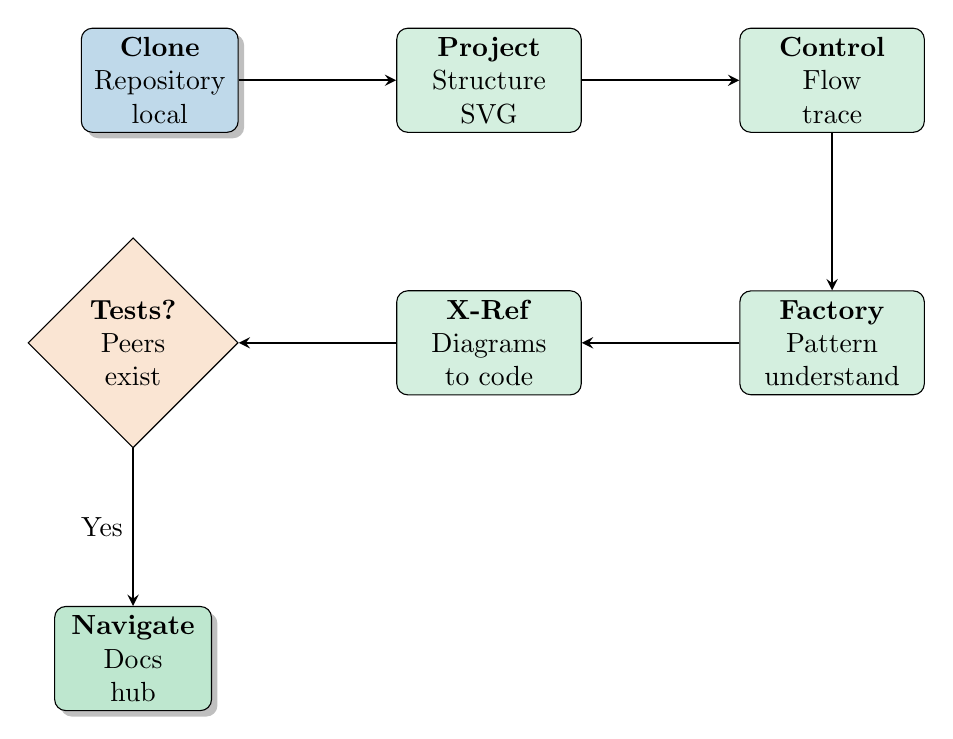
\begin{tikzpicture}[node distance=2cm, auto]
    \node[block, fill=primary!30] (clone) {\textbf{Clone}\\Repository\\local};
    \node[process, right=of clone] (project) {\textbf{Project}\\Structure\\SVG};
    \node[process, right=of project] (control) {\textbf{Control}\\Flow\\trace};
    \node[process, below=of control] (factory) {\textbf{Factory}\\Pattern\\understand};
    \node[process, left=of factory] (xref) {\textbf{X-Ref}\\Diagrams\\to code};
    \node[decision, left=of xref] (tests) {\textbf{Tests?}\\Peers\\exist};
    \node[block, fill=secondary!30, below=of tests] (nav) {\textbf{Navigate}\\Docs\\hub};

    \draw[arrow] (clone) -- (project);
    \draw[arrow] (project) -- (control);
    \draw[arrow] (control) -- (factory);
    \draw[arrow] (factory) -- (xref);
    \draw[arrow] (xref) -- (tests);
    \draw[arrow] (tests) -- node[left] {Yes} (nav);
\end{tikzpicture}
\end{center}

\begin{itemize}
  \item[$\square$] \textbf{Clone Repository}: Get local copy of diagrams
  \item[$\square$] \textbf{Project Structure}: Open \texttt{docs/diagrams/project\_structure.svg}
  \item[$\square$] \textbf{Control Flow}: Trace execution path in \texttt{control\_flow.svg}
  \item[$\square$] \textbf{Factory Pattern}: Understand controller instantiation
  \item[$\square$] \textbf{Cross-Reference}: Match diagram nodes to \texttt{src/} files
  \item[$\square$] \textbf{Test Peers}: Verify every \texttt{src/*.py} has \texttt{tests/test\_*.py}
  \item[$\square$] \textbf{Documentation Hub}: Explore \texttt{docs/NAVIGATION.md}
  \item[$\square$] \textbf{Architecture Guide}: Read \texttt{CLAUDE.md} Section 25 (standards)
\end{itemize}

% =============================================================================
% NEXT STEPS
% =============================================================================
\section*{Next Steps}
\begin{itemize}
  \item \textbf{E024}: Lessons learned and best practices (6-month retrospective)
  \item \textbf{E025-E029}: Appendix reference (5-part technical deep dive)
\end{itemize}

\end{document}
